\section{Introduction}
\label{sec:intro}

The energy consumption due to buildings (both residential and commercial)
is estimated to be 20\% to 40\% of the total energy usage in
developed countries~\cite{pop08}, and
lighting and heating are two significant components of this energy
consumption~\cite{keh05}.
Natural light (i.e., sunlight) is a readily available resource that
can contribute to both the illumination and heating of structures,
yet in the vast majority of circumstances, its use is limited to
passive modalities.  For example, daylighting (the use of natural
light for illumination) design is dominated by passive window positioning
and configuration~\cite{vgf+13} rather than active control mechanisms
(see~\cite{kt16} for the few counterexamples).

\FIXME{What are we doing?}

Figure~\ref{fig:amp} is an image of a prototype catoptric (mirror) surface
(called AMP) that was designed, fabricated, and installed through an
undergraduate architecture studio taught by C.~Ahrens. The installation
redirects light from gable ends of an existing building into the darker
recesses of the atrium to create better natural lighting where it is desired.
In this installation, the mirror positions are fixed.

\begin{figure}[ht]
\centering
\subfloat[\mbox{ }]{

\includegraphics[width=0.5\linewidth]{figures/amp}
\label{fig:amp}}
\qquad \qquad
\subfloat[\mbox{ }]{
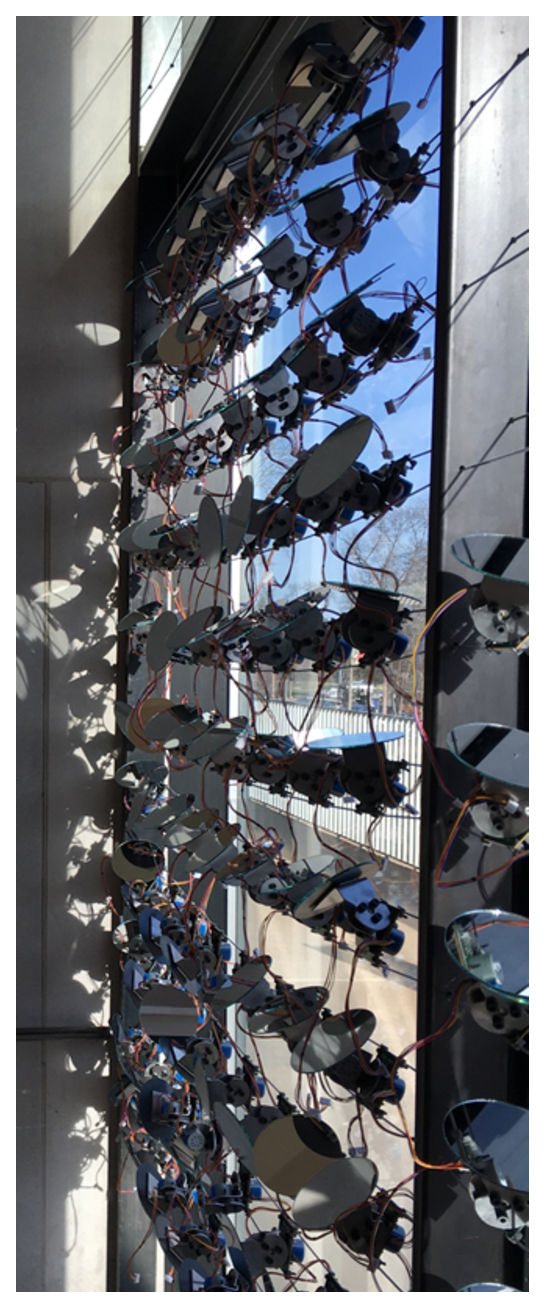
\includegraphics[width=0.16\linewidth]{figures/steinberg}
\label{fig:steinberg}}
\caption{Catroptic system prototypes.
(a)~\emph{AMP}, TRex building, St. Louis, MO.
(b)~\FIXME{name?}, Steinberg Hall, St. Louis, MO.
}
\label{fig:proto}
\end{figure}

In the next generation of this system, which is currently under construction,
the mirrors are under active, 2-axis, microprocessor-based control and
therefore can be pointed in different directions dynamically as desired
over time.



\FIXME{Where (if at all) should we define Open-Source Architecture (OSArc) as
distinct from open-source software? How do the notions of OSArc integrate
with what we are doing? (This is a Chandler question.) Is~\cite{BS13} a
good citation (I just found it on wikipedia)? How about one or more things that
Chandler has written?}

\FIXME{Articulate specific research questions below.}

This research will investigate the following questions:
\begin{enumerate}

\item \emph{What are the qualitative and quantitative benefits
that can be achieved for bulding daylighting and thermal management
through the use of catoptric systems?}

Issues within this question include \FIXME{talk about multi-objective control
in an MDP framework}.

\item \emph{How do we provide for the safety, reliability, maintainability, and
continued efficacy of these systems?}

\item \emph{Can we design abstractions that encapsulate sub-systems for
effective reuse?}
Ultimately, we would like to generalize the above into abstractions that can be
leveraged more broadly for arbitrary cyber-physical systems development.

\end{enumerate}

\FIXME{Brief description of who we are and what we've done.}
